\subsection{Revving the VIPUR approach to expand rare disease diagnostics}
	\subsubsection{Preparatory steps for using the VIPUR approach}
		After the publication of VIPUR the tools, data and applications became available at the open science framework (OSF) \cite{} which were downloaded and reviewed. All applications from the Rosetta software suite (Section \ref{subsec:MM_Rosetta}) were pre-compiled without support for MPI (Section \ref{subsec:MM_MPI}) and with that not the ability to benefit from multiple CPUs. The Rosetta software suite was rebuilt with MPI support in a slurm job where the compilation could benefit from multiple CPU cores.
		%VIPUR: Variant Interpretation and Prediction Using Rosetta, Baugh
	\label{subsubsec:RES_Prepare}
	
	\subsubsection{VIPUR resolving system incompatibilities}
	Within the VIPUR pipeline residues were mutated to determine the effects of a structural mutation, by default missense mutations were inserted with PyMOL (Section \ref{subsec:MM_PyMOL}), an alternative method integrated within the pipeline for situations wherein PyMOL was not accessible Pyrosetta (Section \ref{subsec:MM_PyRosetta}) could be used. Neither of these programs could be built or compiled because the lack of Open graphics library (OpenGL) for PyMOL and having the incorrect C++ and C libraries for PyRosetta. To bypass both programs and still be able to introduce mutations into PDB files Modeller (Secton \ref{subsec:MM_Modeller}) was introduced and built.
	
	\begin{figure}[!ht]
		\centering
		\begin{subfigure}{0.45\textwidth}
			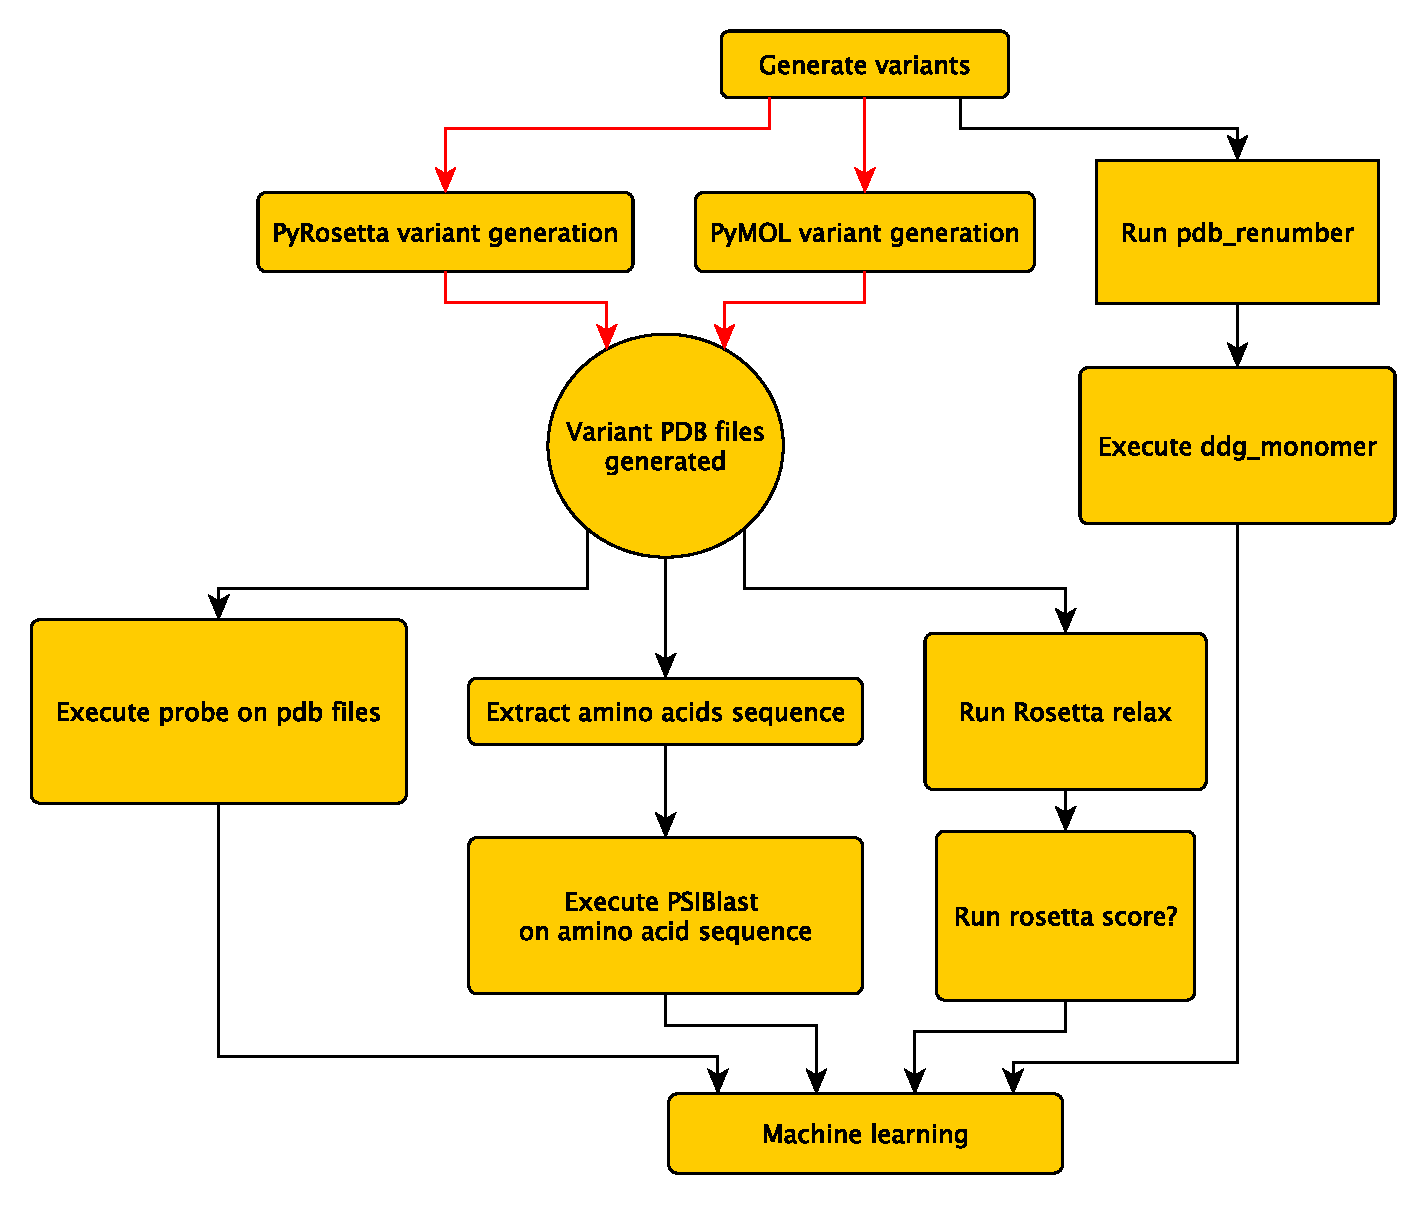
\includegraphics[width=\textwidth]{Flowcharts/VIPUR_approach.pdf}{a}
			\phantomcaption
			\label{fig:RES_VIPUR_approach}
		\end{subfigure}
		\begin{subfigure}{0.45\textwidth}
			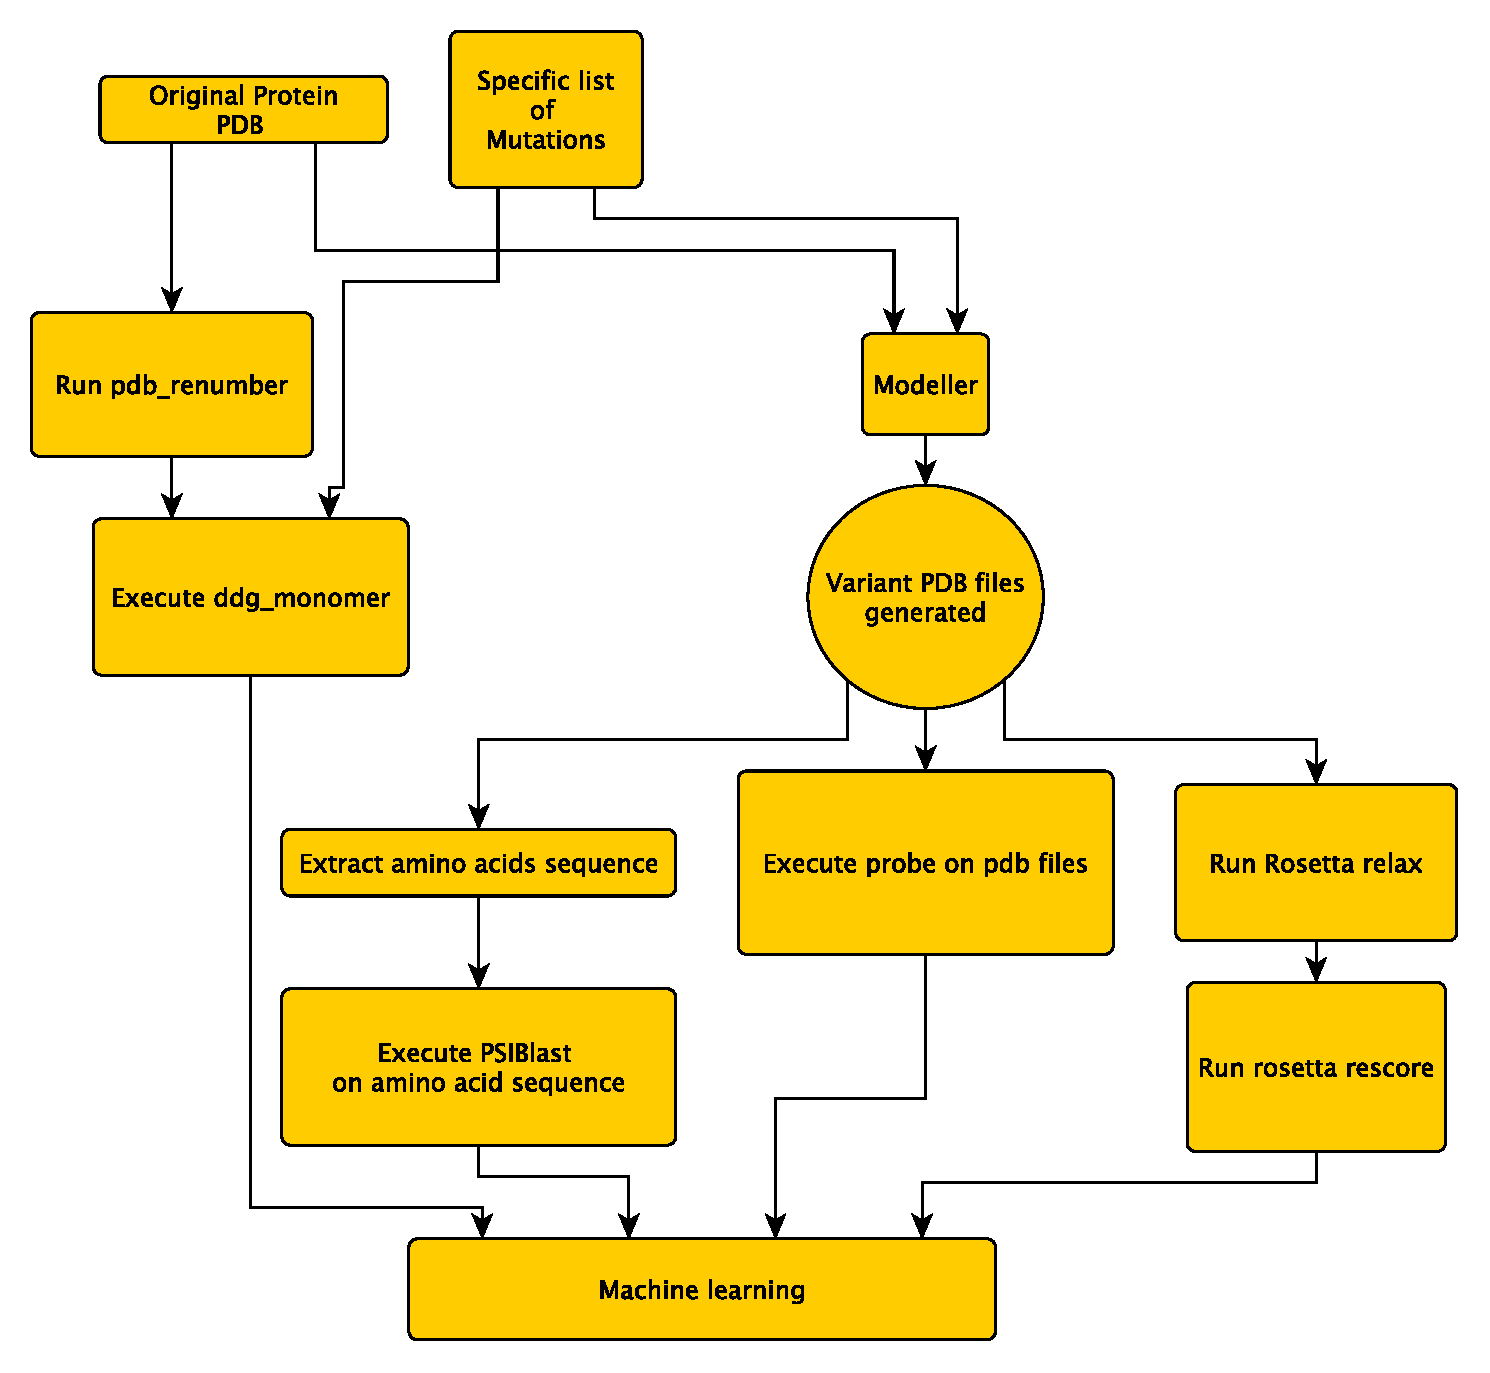
\includegraphics[width=\textwidth]{Flowcharts/Altered_VIPUR_approach.pdf}{b}
			\phantomcaption
			\label{fig:RES_Altered_VIPUR_approach}
		\end{subfigure}
		\caption[Flowcharts VIPUR pipeline and altered VIPUR pipeline]{Both flowcharts illustrate the VIPUR pipeline wherein each block is a procedure the central circle is the purpose of the mutated applications and each arrow represents the path to it. Figure \ref{fig:RES_VIPUR_approach} has red arrows that indicate that both methods were incapable to produce the mutated PDB files. Within figure \ref{fig:RES_Altered_VIPUR_approach} the alternative method is proposed wherein PyMOL and PyRosetta (Sections \ref{subsec:MM_PyMOL}, \ref{subsec:MM_PyRosetta}) is substituted by Modeller (Section \ref{subsec:MM_Modeller}) to acquire the mutated protein structures.}

		\label{fig:Flowcharts_of_old_and_altered_VIPUR}
	\end{figure}
	\label{subsubsec:RES_Incompatibility}
	\newpage
	
	\subsubsection{Expanding the VIPUR training set with data from TNFRSF1A by homology modeling and protein threading}
	Since the VTS did not have any features of TNFRSF1A (Section \ref{subsec:CD_TNFRSF1A}) the amino acid sequence was collected from Uniprot (Section \ref{subsec:MM_Uniprot}) and the protein from RCSB (Section \ref{subsec:MM_RCSB}). The structures available of TNFRSF1A were incomplete, fragments for the TNF $\alpha$ and $\beta$ binding site \cite{} were available and its death domain that interacts with TRADD \cite{} which plays a role in apoptosis (Section \ref{subsec:CD_TNFRSF1A}). To acquire a monomeric structure of TNFRSF1A two ab initio modeling web services I-TASSER and Robetta (Sections \ref{subsec:MM_I_TASSER}, \ref{subsec:MM_Robetta}) had been employed. Both were given the task to model the whole protein with and without a template to determine how well they could model a known structure and what it would form. Determination of the best model was based on the smallest root mean square deviation distance (RMSD )in {\AA} , between a produced model compared to the X-ray crystallographic model of the TNFRSF1A binding site .
	
%	Solution structure of the tumor necrosis factor receptor-1 death domain, Sukits
	\begin{figure}[!ht]
		\centering
		\begin{subfigure}{0.45\textwidth}
			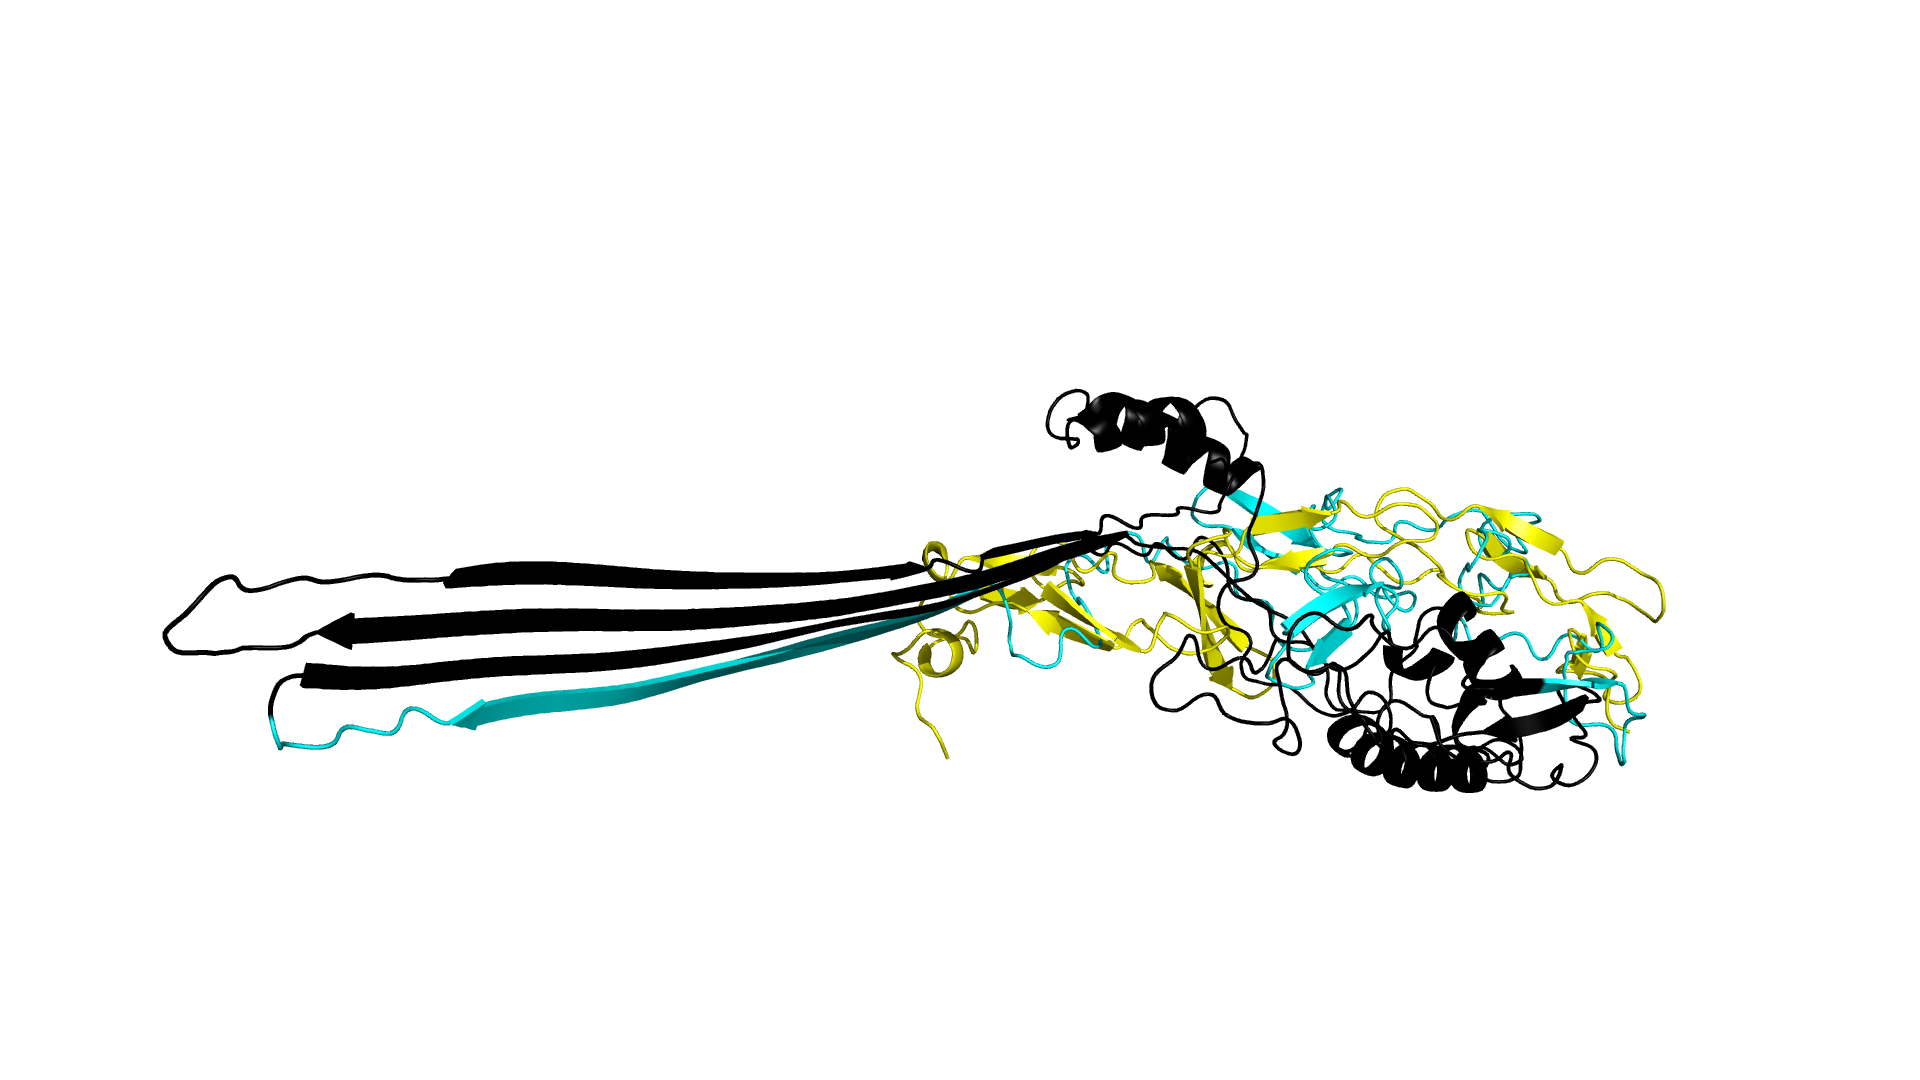
\includegraphics[width=\textwidth]{I_TASSER_Robetta_Images/1_EXT_ALIGN_I_TAS_WITHOUT_TEMPLATE.png}{a}
			\caption{RMSD = {\AA} 28.786}
			\label{fig:RES_I_TASSER_Without}
		\end{subfigure}
		\begin{subfigure}{0.45\textwidth}
			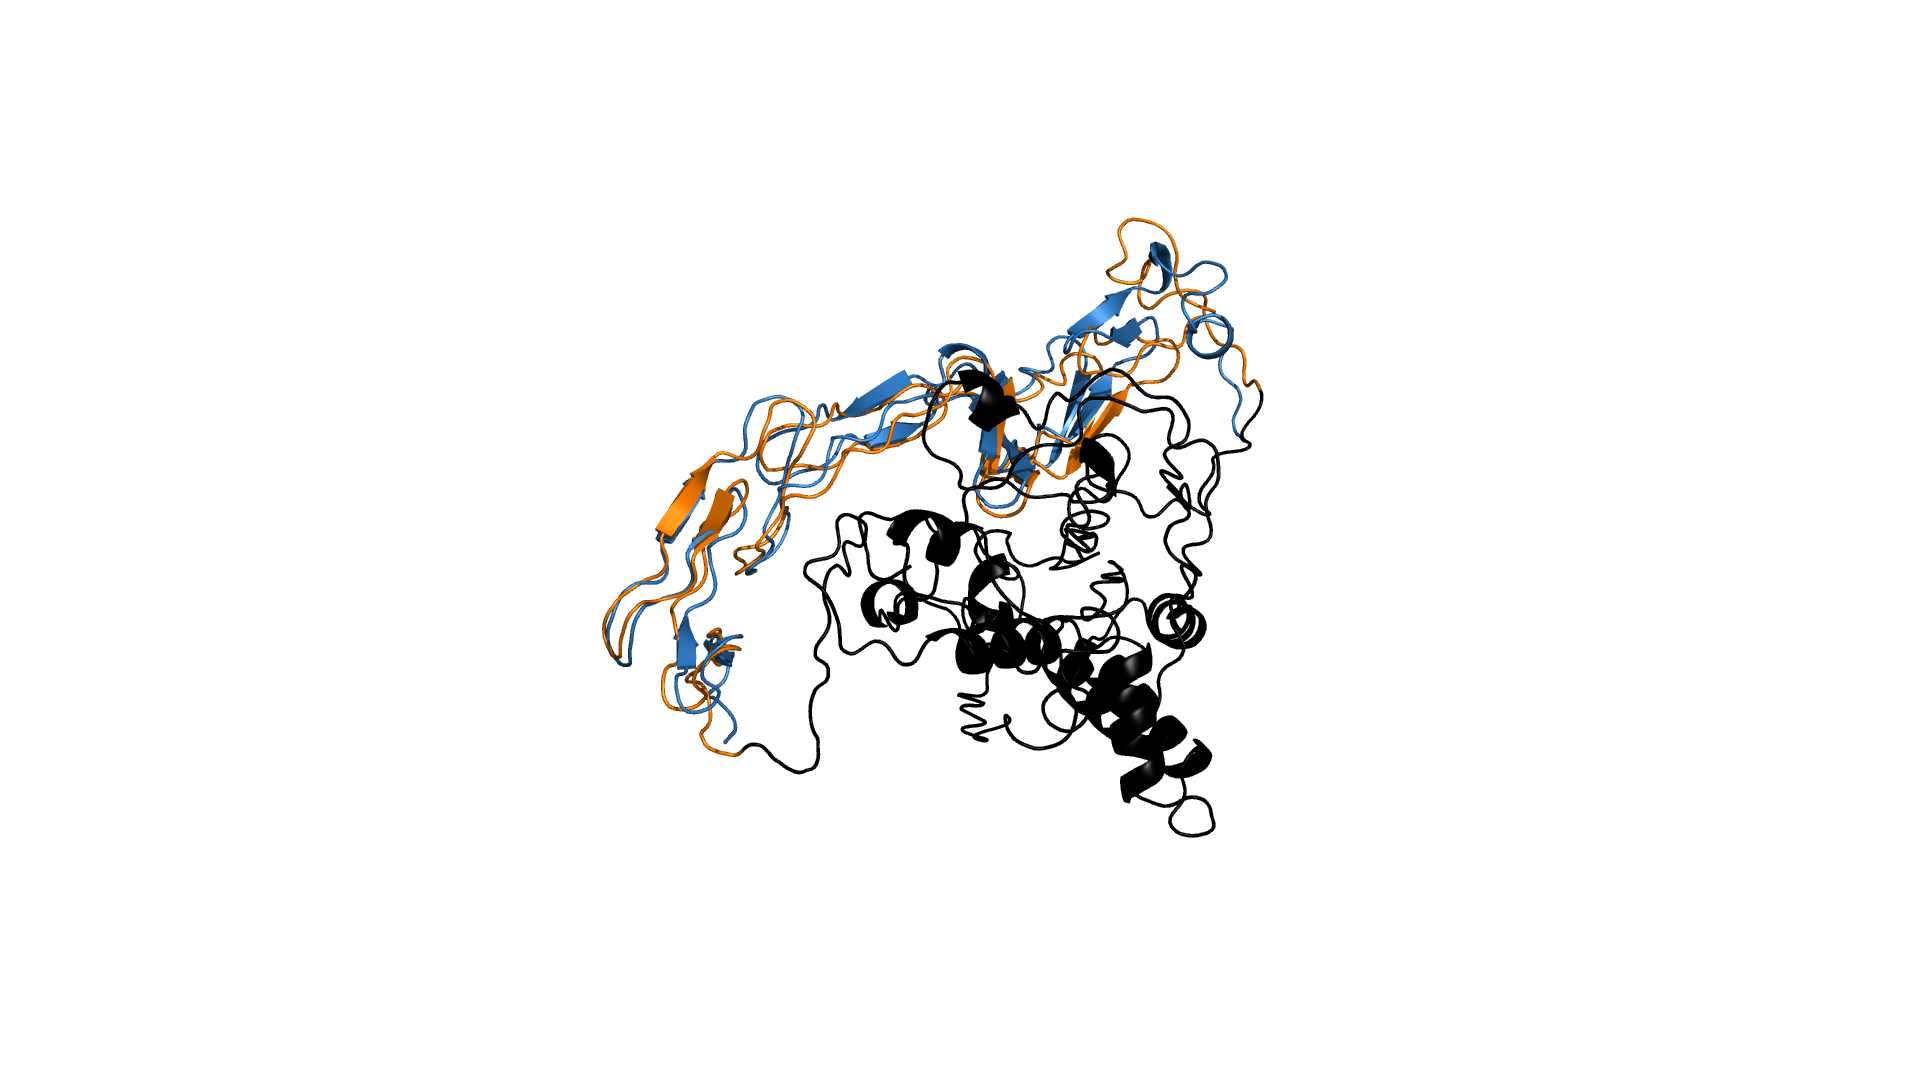
\includegraphics[width=\textwidth]{I_TASSER_Robetta_Images/1_EXT_ALIGN_I_TAS_WITH_TEMPLATE.png}{b}
			\caption{RMSD = {\AA} 3.830}
			\label{fig:RES_I_TASSER_With}
		\end{subfigure}
		\begin{subfigure}{0.45\textwidth}
			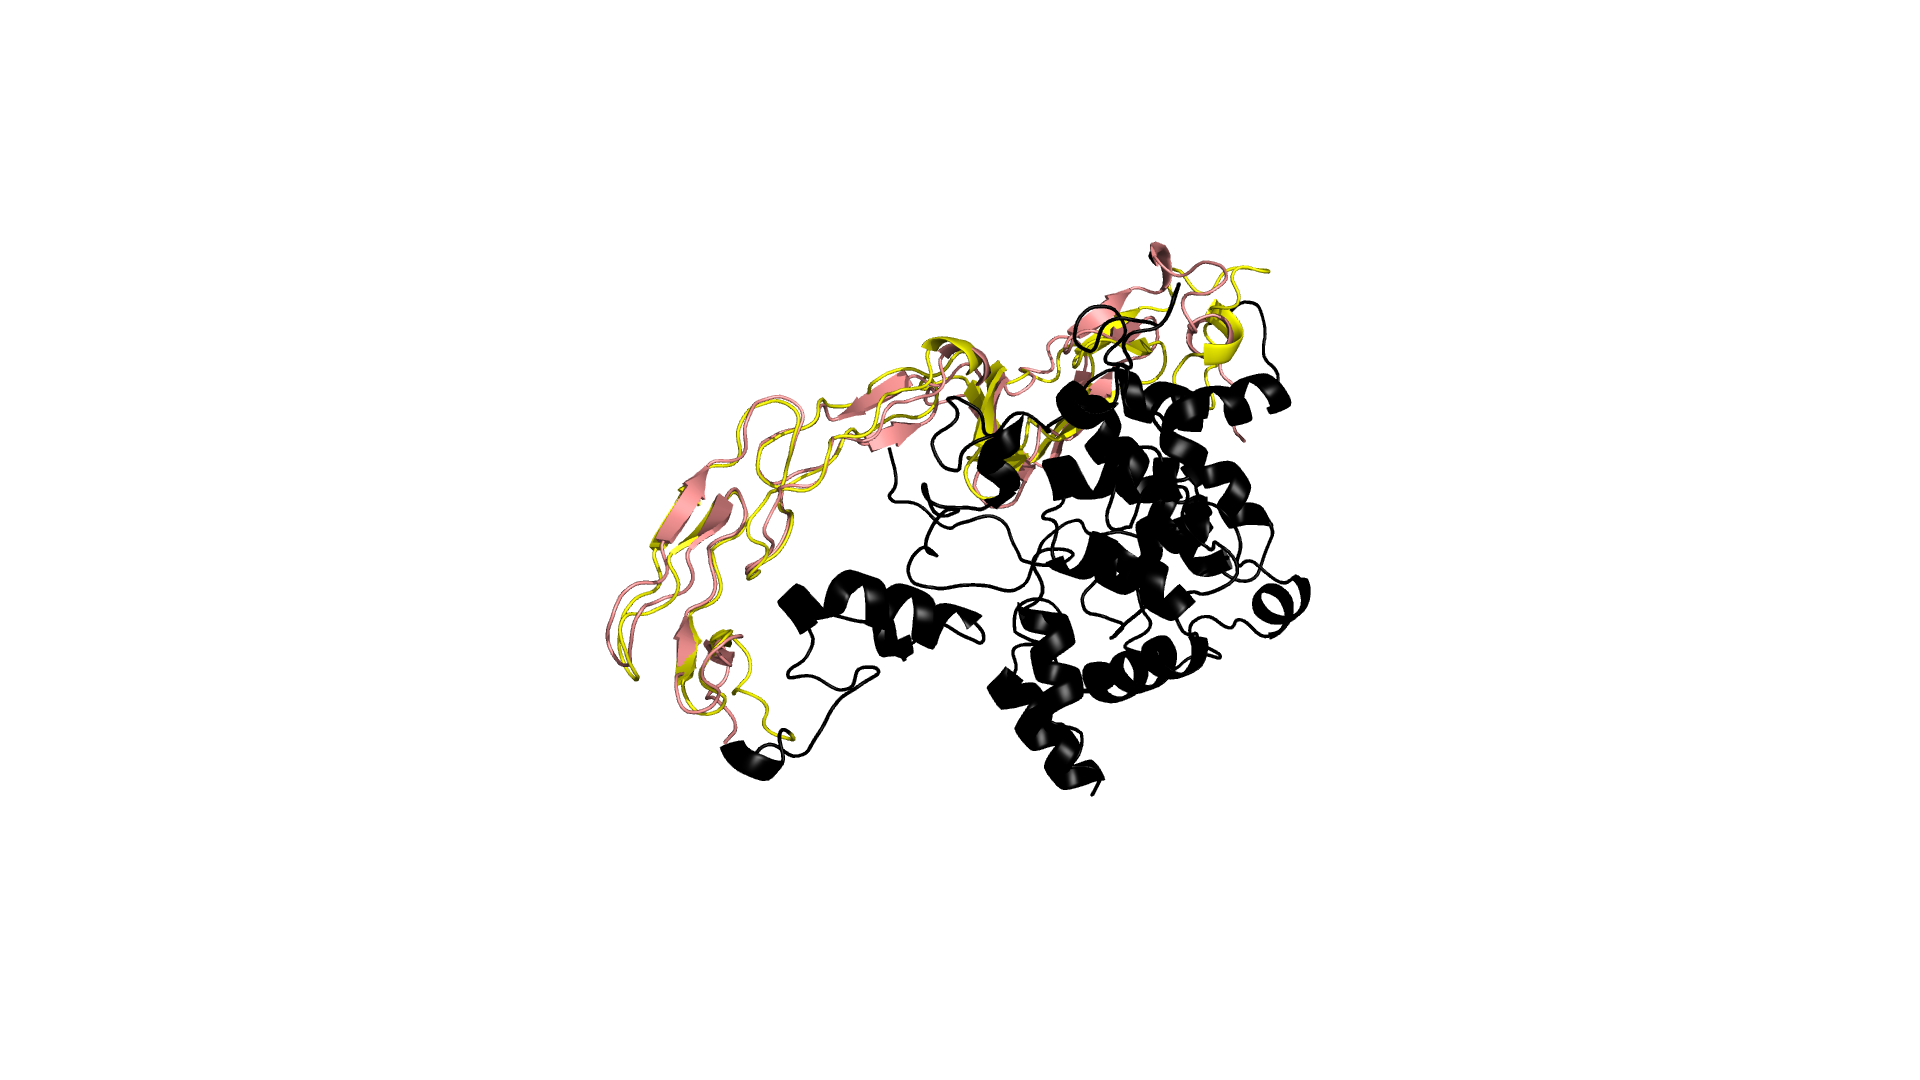
\includegraphics[width=\textwidth]{I_TASSER_Robetta_Images/1_EXT_ALIGN_ROB_WITHOUT_TEMPLATE.png}{c}
			\caption{RMSD =  {\AA} 3.067}
			\label{fig:RES_Robetta_Without}
		\end{subfigure}
		\begin{subfigure}{0.45\textwidth}
			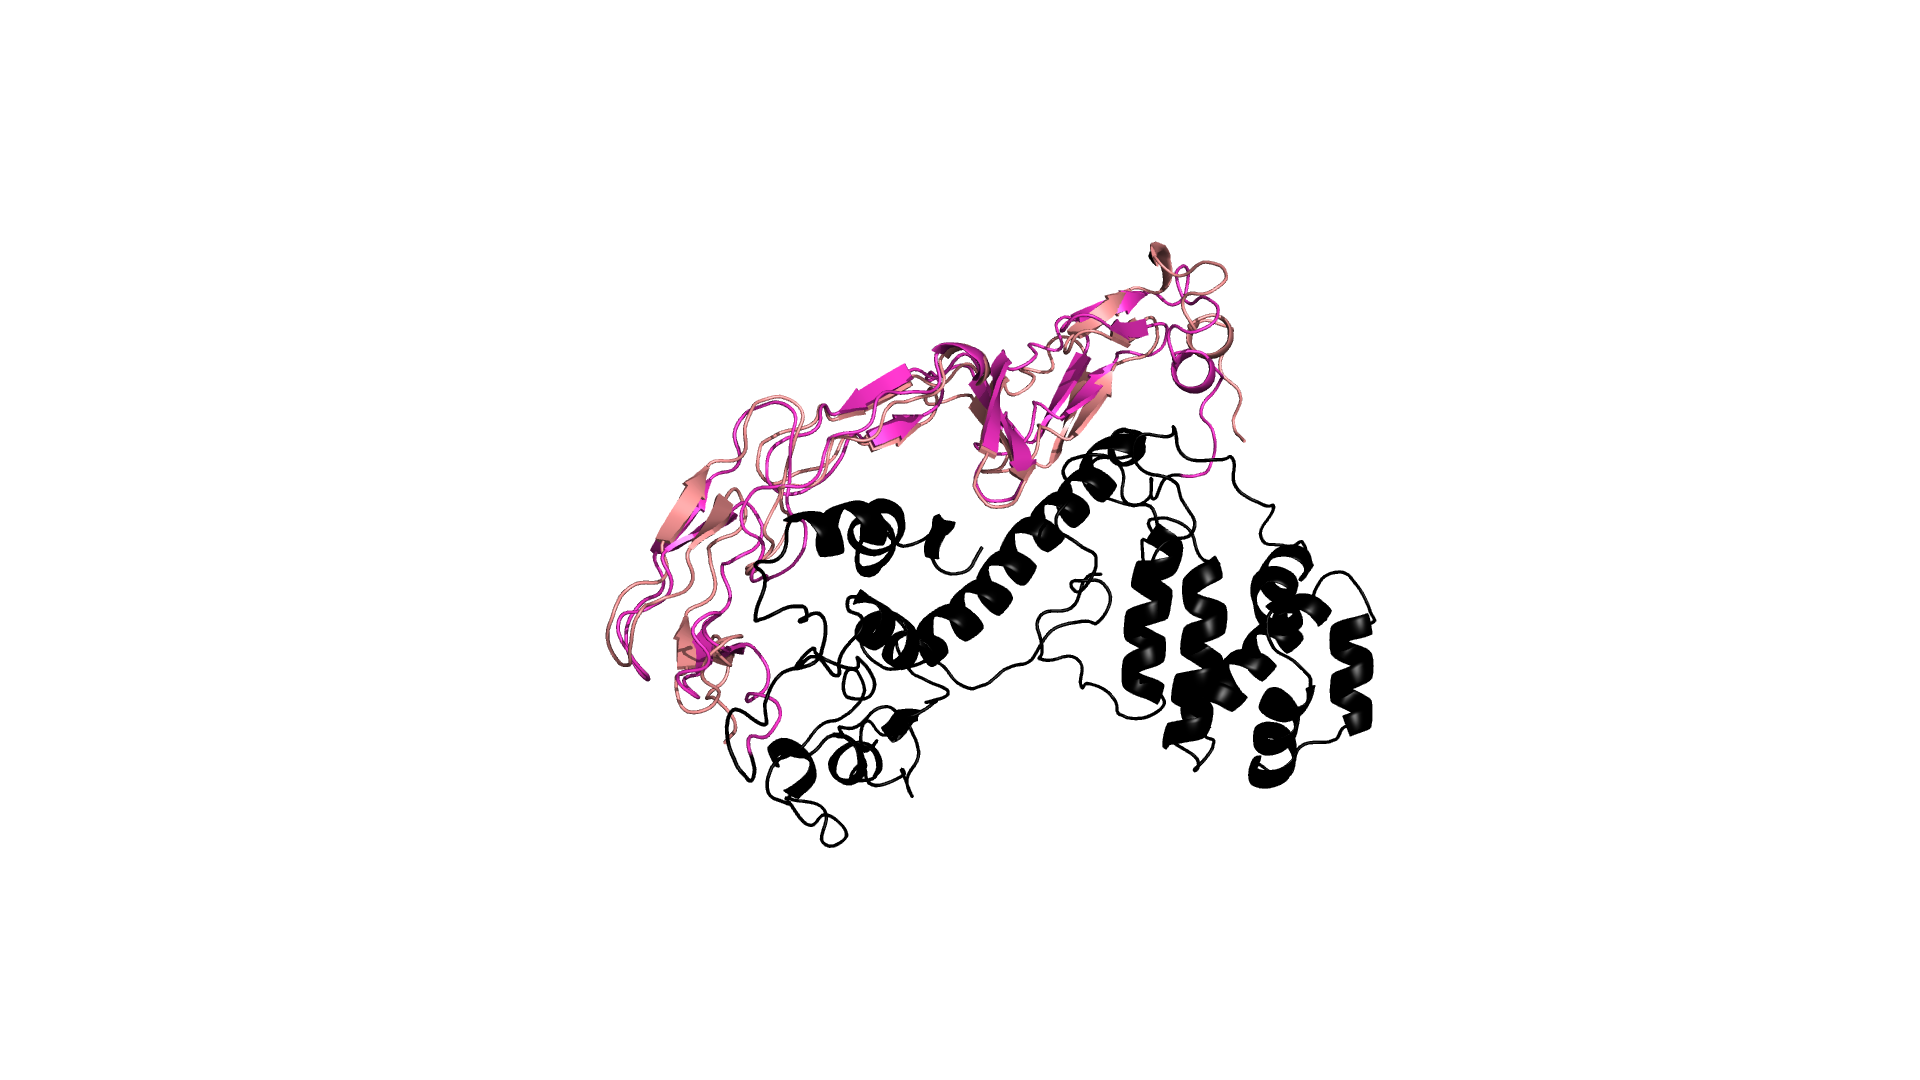
\includegraphics[width=\textwidth]{I_TASSER_Robetta_Images/1_EXT_ALIGN_ROB_WITH_TEMPLATE.png}{d}
			\caption{RMSD =  {\AA} 2.877}
			\label{fig:RES_Robetta_With}
		\end{subfigure}
		\caption[I-TASSER and Robetta models with and without templates]{3D structures of TNFRSF1A ( \ref{fig:RES_I_TASSER_Without}, \ref{fig:RES_I_TASSER_With}: I-TASSER, \ref{fig:RES_Robetta_Without}, \ref{fig:RES_Robetta_With}: Robetta) without (left: \ref{fig:RES_I_TASSER_Without}, \ref{fig:RES_Robetta_Without}) and with templates (right: \ref{fig:RES_I_TASSER_With}, \ref{fig:RES_Robetta_With}). The sky blue colored structure in each figure is an X-ray crystallographic model (1EXT) of the binding site of TNFRSF1A and the orange structure is the representation of that identical fragment in the model made by the web services.}
	\end{figure}
	\label{subsubsec:RES_Expanding_Models}

\newpage
\subsection{Analyses of proteins variants TNFRSF1A}
	\subsubsection{Requirements for determining structural and binding effects of protein variants}
	Protein variants can be assessed from multiple perspectives and together they can form a holistic view on how a protein works and how mutations affect its workings. However adding perspectives to the protein assessment makes it complex and requires expertise to determine its validity and contribution, therefore the analysis has been limited to basic structural information and also make the assessment inline with the VIPUR methods.
	
	Various proteins consist of multiple chains that can be identical or different depending on their function \cite{} and should be taken into account when assessing protein variants since one residue might alter the binding between chains and might alter the proteins formation. 
%	Lipin proteins form homo- and hetero-oligomers, Liu et al.
	Different molecules and atoms that do not make up a protein but play a role in a pathway and function (ligands and co-receptors) are able to affect a proteins shape and can behave differently when a residue is mutated. 
	
	A different aspect that can change with mutations is the alteration in motions between structures which can allow or disallow certain movements to occur and with inhibit processes.
	
%	In context of TNFRSF1A dimers that are formed when unbound can be altered by mutations and 
	
%	Other parts that alter to protein and play a role in function are ligands and co-receptors that 
%	To get the appropriate structural information of a protein 
%	
%	the informational search scope has been limited to structural information and 
%	
%	 therefore the search scope has been limited to structural information.
%	For structurally assessing protein variants a there are several requirements, 


%	SOMETHING ABOUT 1TNR and 1EXT!
%	Structural information of proteins describes how a protein functions and how it behaves within a cell, however it is difficult to analyze since
%	
%	Proteins variants can be assessed from different perspectives and all are necessary to 
%	Assessing protein variants and its effects 
%	
%	Assessing protein variants and the effects that a variant might cause can be assessed from different fields of view and could give a holistic view on problem that arise during mutations. However adding every perspective in an analyses is difficult because collecting all available information often has to be done manually and to determine which information is relevant requires expertise. However it can be complex to put all the information and since  
%	
%	
%	Because the VTS mainly consists of structural features and 
%	
%	To make assessment less complex and because the VTS has mainly structural features 
%	
%	 a structural point of view was taken for the protein TNFRSF1A 
%	
%	To simplify the complexity of the problem only a structural point of view with limited alterations was taken
%	
%	To simplify the problem it has been recapitulated into 
%	
%	the perspectives of form and function.
%	
%	The perspective of form describes how a protein takes shape based on the environment and amino acid sequence, within the context of TNFRSF1A it describes how dimer structures are formed on the cell surface when unbound and that it forms a trimeric structure when it is bound by TNF 
%	
%	Function determines how certain parts of a protein behave within an environment and determine its effects on a pathway. 
%	
%	In context with TNFRSF1A one part resides on the cell surface where it binds ligands and on the cytoplasmic side it can interact with protein that triggers an inflammatory response or apoptosis. When a mutation is introduced at the cell surface side it might not be able to form dimer formations that interact with TNF ligands or during transformation with the binding of TNF it is unable to bind trimers. 
%	
%	Wherein the perspective of form the deciding factors are the amino acid sequence and where it resides within the cell.
%	
%	A different perspective is form wherein the amino acid sequence determines how a protein structure will be formed.
%	
%	Before the moment of writing no protocol was available which dealt with structural variation 
%	
%	Currently there is no protocol available to asses protein variants with structural information, 
	
%	Assessing protein variants and its effects should be studied with a multidisciplinary view wherein form and function are assessed. Within the aspect of form should be seen how a protein is formed
%	
%	
%	However due to difficulties with experiments it can be hard to unravel all the effects that can be caused by mutations.
%	
%	 A part of this view is to know what function the protein has before its mutated to determine its effect on a pathway or function. 
%	
%	How does the 
%	
%	
%%	 Effect
%	Can a cell or pathway still function without this protein? or is there an alternative mechanism within the cell that is less efficient in performing similar role? 
	
	\subsubsection{Single protein variant analysis approach and its tools}
	Before introducing mutations into a protein structure it is helpful to know if a mutation has been observed to avoid allocating resources to something that does not occur. Therefore three tables with observed TNFRSF1A mutations (Sections \ref{subsec:MM_GAVIN_data_table}, \ref{subsec:MM_GnomAD}, \ref{subsec:MM_Infevers}) have been combined with an R script (Section \ref{subsec:MM_R}) into a single table consisting of two columns. The first column (split into three columns \ref{table:Res_Filtered_Mutations}) contains strings that describes the: original residue, position and where it mutates to, the second column describes whether a formed mutation is harmful, with most mutations the effects have not been identified yet. 
	\begin{table}[ht]
		\begin{tabular}{ l | l | l | l}
			Original residue & Position in the protein sequence & New residue & Classification\\ \hline
			Cys & 44 & Tyr & PATHOGENIC\\
			Thr & 44 & Pro & PATHOGENIC\\
			Thr & 44 & Ser & PATHOGENIC\\
		\end{tabular}
		\caption[Sample of combined tables with observed mutations]{The format wherein mutations were filtered from the GAVIN, GenomAD and Infevers tables (Sections \ref{subsec:MM_GAVIN_data_table},  \ref{subsec:MM_GnomAD}, \ref{subsec:MM_Infevers}),  describe whether a structural mutation is harmful or not. For many mutations it is unknown and other classifications are available, to view the whole table visit the supplementary.}
		\label{table:Res_Filtered_Mutations}
	\end{table}
	
	For assessing variants in TNFRSF1A a structural fragment was used that contained TNF $\beta$ (1TNR) \cite{} and was made homotrimeric with PyMOL (Section \ref{subsec:MM_PyMOL}) which results in six chains that emulate a bound TNFRSF1A with TNF $\beta$. The first column of the mutation table did not contain sufficient information to apply mutations correctly and within the PDB different numbering is used than in the amino acid sequence. To bundle the information and make it usable for introducing mutations a Python script (Section \ref{subsec:MM_Python}) has been written that combines the mutation table, PDB chains and the correct position within the sequence into a type of table which has sufficient information to mutate structures.  
	%	Crystal structure of the soluble human 55 kd TNF receptor-human TNFβ complex: Implications for TNF receptor activation, Banner et al. 
	\begin{table}[ht]
		\begin{tabular}{ l | l | l | l | l}
			Iteration number & Filename & Chain & Residue index in chain & New residue\\ \hline
			34 & 1tnr3\_TNFA & R & 0 & TYR\\
			34 & 1tnr3\_TNFA & T & 0 & TYR\\
			34 & 1tnr3\_TNFA & S & 0 & TYR\\
			35 & 1tnr3\_TNFA & R & 0 & PRO\\
			35 & 1tnr3\_TNFA & T & 0 & PRO\\
			35 & 1tnr3\_TNFA & S & 0 & PRO\\
			36 & 1tnr3\_TNFA & R & 0 & SER\\
			36 & 1tnr3\_TNFA & T & 0 & SER\\
			36 & 1tnr3\_TNFA & S & 0 & SER\\
		\end{tabular}
		\caption[Sample of table with missense mutations applicable to TNFRSF1A PDB]{The format that describes the mutations that should be made by Modeller (Section \ref{subsec:MM_Modeller}), with specifications of the: model, file. chain, residue index and the new residue. The whole table for TNFA and TNFB are visible within the supplementary.}
			\label{table:Res_Modeller_Mutation_Format}
	\end{table}
	
	\newpage
	To introduce mutations within PDB structures a Python script (Section \ref{subsec:MM_Python}) was written which used the generated mutation table (Table: \ref{table:Res_Modeller_Mutation_Format}) and a matching PDB structure, from the table; it acquires an iteration number which specifies if a mutation has to be stored in a single file or across multiple files; the filename serves as key which determine the PDB that should be used; letters specify chains, numbers are indices within the chains and the last column states the three letter residue where it should mutate to. When a structure is read in through the Python bindings of Modeller (Section \ref{subsec:MM_Modeller}) all non standard atoms and molecules are removed because Rosetta (Section \ref{subsec:MM_Rosetta}) is not able to deal with those atoms. Just before mutagenesis takes place missing atoms are added to the structure that were difficult to determine with experimental methods(Section \ref{subsec:GD_Addition_of_structural_data}). After the insertion of all mutations a last guess is made where disulfide bonds are added between cysteines. With this process variants can be easily made, however the mutations do not present a correct protein because the mutated residues can put the protein in a high energy state.
	
	In the attempt to make mutated structures behave more natural two tools from the Rosetta software suite (Section \ref{subsec:MM_Rosetta}) have been used to minimize energies within protein structures. With the backrub application (Section \ref{subsubsec:MM_Backrub}) 1000 altered backbone models have been produced each with 10000 Monte Carlo moves (Sections \ref{section:Chap_Monte_Carlo}). Each model generated has a set of properties that describe the formed molecule 
	
	Relax **
	
	We specifically chose to asses known mutations from infevers. **
	Density goes beyond 1 ***
	
\newpage	
\subsection{Finding structural information and its mutations through HOPE}
	With uncertainty in the numbers provided by SPVAA a more textual informative approach was used with the web service HOPE (Section \ref{subsec:MM_HOPE}). The mutations that were known from Infevers (Section \ref{subsec:MM_Infevers}) and were also used with SPVAA were tested by HOPE (CYS62GLY, GLU138ALA and PHE141IlE), all reports are visible within the supplementary.
	
	HOPEs first test was the mutation of Cysteine 62 to glycine, which is known within the Infevers table as pathogenic. It discovered that the residue was involved in a disulfide bridge and was 100\% conserved in related protein sequences, based on the observation that cysteine formed a disulfide bridge it expected that with te replacement of it glycine would make the whole structures less rigid. HOPE predicts that mutation is pathogenic because of the high conservation of the residue, which is further confirmed by its search results in which if found the original publication where the observation has been described and associated to TRAPS \cite{}.
%	The tumor-necrosis-factor receptor-associated periodic syndrome: new mutations in TNFRSF1A, ancestral origins, genotype-phenotype studies, and evidence for further genetic heterogeneity of periodic fevers, Aksentijevich
	
	According to Infevers is the mutation of glutamic acid at position 138 mutated to alanine classified as likely benign, HOPE discovered with its BLAST query that glutamic acid occurs the most often at position but other residues such as alanine have been observed at the position. Structurally glutamic acid forms salt bridges with proline  368 and leucine 390, it lies within a part which is repeated and used for binding, it might already perturb the binding capabilities according to HOPE.
	
	
%	
%	
%	 to arrange this information properly a Python script (Section \ref{subsec:MM_Python}) used the files and
%	
%	 and the exact position within the PDB file (1TNR) had to be added with a Python script (Section \ref{})
%	
%	 were introduced with a Python script (Section \ref{subsec:MM_Python}) wherein  and had to be introduced with  Introducing mutations in the trimeric mol
%	
%	Each of wherein mutated 
%	
%	
%	
%	three mutations in separate structures were introduced.
%	
%	The mutation tables first column is insufficient and requires additional information regarding TNFRSF1A chains to make mutations in TNFRSF1A, information regarding the chains 
%	
%	From the mutation table only information of the first column is used to make alterations in structural models, that part of the table will play a role in modifying protein structures with Modeller (Section \ref{subsec:MM_Modeller}). Because the model is homotrimeric it has multiple poly peptides chains that all need to be modified without modifying the ligand. 
%	
%		
%	
%	 But more information is required to make a new format, since TNFRSF1A is a homotimer a
%	the function of the mutated protein is within a pathway 
%	A broad perspective should be taken with a 
%	To determine the effects of mutated residue awithin a protein variant a b than structural information should
%	Up until VIPUR and the development of similar approaches that benefit from structural information

%
%
%
%Something about that we tried to use the VTS and add our protein for information.



